\documentclass[1p]{elsarticle_modified}
%\bibliographystyle{elsarticle-num}

%\usepackage[colorlinks]{hyperref}
%\usepackage{abbrmath_seonhwa} %\Abb, \Ascr, \Acal ,\Abf, \Afrak
\usepackage{amsfonts}
\usepackage{amssymb}
\usepackage{amsmath}
\usepackage{amsthm}
\usepackage{scalefnt}
\usepackage{amsbsy}
\usepackage{kotex}
\usepackage{caption}
\usepackage{subfig}
\usepackage{color}
\usepackage{graphicx}
\usepackage{xcolor} %% white, black, red, green, blue, cyan, magenta, yellow
\usepackage{float}
\usepackage{setspace}
\usepackage{hyperref}

\usepackage{tikz}
\usetikzlibrary{arrows}

\usepackage{multirow}
\usepackage{array} % fixed length table
\usepackage{hhline}

%%%%%%%%%%%%%%%%%%%%%
\makeatletter
\renewcommand*\env@matrix[1][\arraystretch]{%
	\edef\arraystretch{#1}%
	\hskip -\arraycolsep
	\let\@ifnextchar\new@ifnextchar
	\array{*\c@MaxMatrixCols c}}
\makeatother %https://tex.stackexchange.com/questions/14071/how-can-i-increase-the-line-spacing-in-a-matrix
%%%%%%%%%%%%%%%

\usepackage[normalem]{ulem}

\newcommand{\msout}[1]{\ifmmode\text{\sout{\ensuremath{#1}}}\else\sout{#1}\fi}
%SOURCE: \msout is \stkout macro in https://tex.stackexchange.com/questions/20609/strikeout-in-math-mode

\newcommand{\cancel}[1]{
	\ifmmode
	{\color{red}\msout{#1}}
	\else
	{\color{red}\sout{#1}}
	\fi
}

\newcommand{\add}[1]{
	{\color{blue}\uwave{#1}}
}

\newcommand{\replace}[2]{
	\ifmmode
	{\color{red}\msout{#1}}{\color{blue}\uwave{#2}}
	\else
	{\color{red}\sout{#1}}{\color{blue}\uwave{#2}}
	\fi
}

\newcommand{\Sol}{\mathcal{S}} %segment
\newcommand{\D}{D} %diagram
\newcommand{\A}{\mathcal{A}} %arc


%%%%%%%%%%%%%%%%%%%%%%%%%%%%%5 test

\def\sl{\operatorname{\textup{SL}}(2,\Cbb)}
\def\psl{\operatorname{\textup{PSL}}(2,\Cbb)}
\def\quan{\mkern 1mu \triangleright \mkern 1mu}

\theoremstyle{definition}
\newtheorem{thm}{Theorem}[section]
\newtheorem{prop}[thm]{Proposition}
\newtheorem{lem}[thm]{Lemma}
\newtheorem{ques}[thm]{Question}
\newtheorem{cor}[thm]{Corollary}
\newtheorem{defn}[thm]{Definition}
\newtheorem{exam}[thm]{Example}
\newtheorem{rmk}[thm]{Remark}
\newtheorem{alg}[thm]{Algorithm}

\newcommand{\I}{\sqrt{-1}}
\begin{document}

%\begin{frontmatter}
%
%\title{Boundary parabolic representations of knots up to 8 crossings}
%
%%% Group authors per affiliation:
%\author{Yunhi Cho} 
%\address{Department of Mathematics, University of Seoul, Seoul, Korea}
%\ead{yhcho@uos.ac.kr}
%
%
%\author{Seonhwa Kim} %\fnref{s_kim}}
%\address{Center for Geometry and Physics, Institute for Basic Science, Pohang, 37673, Korea}
%\ead{ryeona17@ibs.re.kr}
%
%\author{Hyuk Kim}
%\address{Department of Mathematical Sciences, Seoul National University, Seoul 08826, Korea}
%\ead{hyukkim@snu.ac.kr}
%
%\author{Seokbeom Yoon}
%\address{Department of Mathematical Sciences, Seoul National University, Seoul, 08826,  Korea}
%\ead{sbyoon15@snu.ac.kr}
%
%\begin{abstract}
%We find all boundary parabolic representation of knots up to 8 crossings.
%
%\end{abstract}
%\begin{keyword}
%    \MSC[2010] 57M25 
%\end{keyword}
%
%\end{frontmatter}

%\linenumbers
%\tableofcontents
%
\newcommand\colored[1]{\textcolor{white}{\rule[-0.35ex]{0.8em}{1.4ex}}\kern-0.8em\color{red} #1}%
%\newcommand\colored[1]{\textcolor{white}{ #1}\kern-2.17ex	\textcolor{white}{ #1}\kern-1.81ex	\textcolor{white}{ #1}\kern-2.15ex\color{red}#1	}

{\Large $\underline{12n_{0154}~(K12n_{0154})}$}

\setlength{\tabcolsep}{10pt}
\renewcommand{\arraystretch}{1.6}
\vspace{1cm}\begin{tabular}{m{100pt}>{\centering\arraybackslash}m{274pt}}
\multirow{5}{120pt}{
	\centering
	\includegraphics[width=112pt]{../../../GIT/diagram.site/Diagrams/png/2243_12n_0154.png}\\
\ \ \ A knot diagram\footnotemark}&
\allowdisplaybreaks
\textbf{Linearized knot diagam} \\
\cline{2-2}
 &
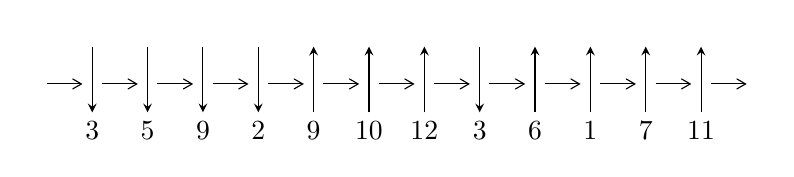
\begin{tikzpicture}[x=20pt, y=17pt]
	% nodes
	\node (C0) at (0, 0) {};
	\node (C1) at (1, 0) {};
	\node (C1U) at (1, +1) {};
	\node (C1D) at (1, -1) {3};

	\node (C2) at (2, 0) {};
	\node (C2U) at (2, +1) {};
	\node (C2D) at (2, -1) {5};

	\node (C3) at (3, 0) {};
	\node (C3U) at (3, +1) {};
	\node (C3D) at (3, -1) {9};

	\node (C4) at (4, 0) {};
	\node (C4U) at (4, +1) {};
	\node (C4D) at (4, -1) {2};

	\node (C5) at (5, 0) {};
	\node (C5U) at (5, +1) {};
	\node (C5D) at (5, -1) {9};

	\node (C6) at (6, 0) {};
	\node (C6U) at (6, +1) {};
	\node (C6D) at (6, -1) {10};

	\node (C7) at (7, 0) {};
	\node (C7U) at (7, +1) {};
	\node (C7D) at (7, -1) {12};

	\node (C8) at (8, 0) {};
	\node (C8U) at (8, +1) {};
	\node (C8D) at (8, -1) {3};

	\node (C9) at (9, 0) {};
	\node (C9U) at (9, +1) {};
	\node (C9D) at (9, -1) {6};

	\node (C10) at (10, 0) {};
	\node (C10U) at (10, +1) {};
	\node (C10D) at (10, -1) {1};

	\node (C11) at (11, 0) {};
	\node (C11U) at (11, +1) {};
	\node (C11D) at (11, -1) {7};

	\node (C12) at (12, 0) {};
	\node (C12U) at (12, +1) {};
	\node (C12D) at (12, -1) {11};
	\node (C13) at (13, 0) {};

	% arrows
	\draw[->,>={angle 60}]
	(C0) edge (C1) (C1) edge (C2) (C2) edge (C3) (C3) edge (C4) (C4) edge (C5) (C5) edge (C6) (C6) edge (C7) (C7) edge (C8) (C8) edge (C9) (C9) edge (C10) (C10) edge (C11) (C11) edge (C12) (C12) edge (C13) ;	\draw[->,>=stealth]
	(C1U) edge (C1D) (C2U) edge (C2D) (C3U) edge (C3D) (C4U) edge (C4D) (C5D) edge (C5U) (C6D) edge (C6U) (C7D) edge (C7U) (C8U) edge (C8D) (C9D) edge (C9U) (C10D) edge (C10U) (C11D) edge (C11U) (C12D) edge (C12U) ;
	\end{tikzpicture} \\
\hhline{~~} \\& 
\textbf{Solving Sequence} \\ \cline{2-2} 
 &
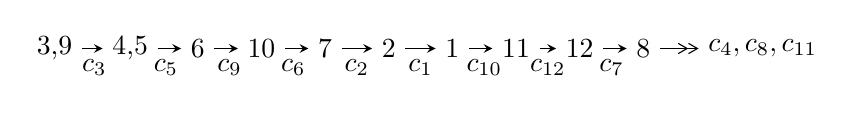
\begin{tikzpicture}[x=23pt, y=7pt]
	% node
	\node (A0) at (-1/8, 0) {3,9};
	\node (A1) at (17/16, 0) {4,5};
	\node (A2) at (17/8, 0) {6};
	\node (A3) at (25/8, 0) {10};
	\node (A4) at (33/8, 0) {7};
	\node (A5) at (41/8, 0) {2};
	\node (A6) at (49/8, 0) {1};
	\node (A7) at (57/8, 0) {11};
	\node (A8) at (65/8, 0) {12};
	\node (A9) at (73/8, 0) {8};
	\node (C1) at (1/2, -1) {$c_{3}$};
	\node (C2) at (13/8, -1) {$c_{5}$};
	\node (C3) at (21/8, -1) {$c_{9}$};
	\node (C4) at (29/8, -1) {$c_{6}$};
	\node (C5) at (37/8, -1) {$c_{2}$};
	\node (C6) at (45/8, -1) {$c_{1}$};
	\node (C7) at (53/8, -1) {$c_{10}$};
	\node (C8) at (61/8, -1) {$c_{12}$};
	\node (C9) at (69/8, -1) {$c_{7}$};
	\node (A10) at (11, 0) {$c_{4},c_{8},c_{11}$};

	% edge
	\draw[->,>=stealth]	
	(A0) edge (A1) (A1) edge (A2) (A2) edge (A3) (A3) edge (A4) (A4) edge (A5) (A5) edge (A6) (A6) edge (A7) (A7) edge (A8) (A8) edge (A9) ;
	\draw[->>,>={angle 60}]	
	(A9) edge (A10);
\end{tikzpicture} \\ 

\end{tabular} \\

\footnotetext{
The image of knot diagram is generated by the software ``\textbf{Draw programme}" developed by Andrew Bartholomew(\url{http://www.layer8.co.uk/maths/draw/index.htm\#Running-draw}), where we modified some parts for our purpose(\url{https://github.com/CATsTAILs/LinksPainter}).
}\phantom \\ \newline 
\centering \textbf{Ideals for irreducible components\footnotemark of $X_{\text{par}}$} 
 
\begin{align*}
I^u_{1}&=\langle 
-1.84711\times10^{54} u^{30}+3.00696\times10^{54} u^{29}+\cdots+1.54890\times10^{57} b+1.97638\times10^{57},\\
\phantom{I^u_{1}}&\phantom{= \langle  }5.87634\times10^{54} u^{30}+8.97726\times10^{53} u^{29}+\cdots+3.09781\times10^{57} a-6.18337\times10^{57},\\
\phantom{I^u_{1}}&\phantom{= \langle  }u^{31}+u^{30}+\cdots+128 u+256\rangle \\
\\
I^v_{1}&=\langle 
a,\;b-1,\;v^8+v^7-3 v^6-2 v^5+3 v^4+2 v-1\rangle \\
\end{align*}
\raggedright * 2 irreducible components of $\dim_{\mathbb{C}}=0$, with total 39 representations.\\
\footnotetext{All coefficients of polynomials are rational numbers. But the coefficients are sometimes approximated in decimal forms when there is not enough margin.}
\newpage
\renewcommand{\arraystretch}{1}
\centering \section*{I. $I^u_{1}= \langle -1.85\times10^{54} u^{30}+3.01\times10^{54} u^{29}+\cdots+1.55\times10^{57} b+1.98\times10^{57},\;5.88\times10^{54} u^{30}+8.98\times10^{53} u^{29}+\cdots+3.10\times10^{57} a-6.18\times10^{57},\;u^{31}+u^{30}+\cdots+128 u+256 \rangle$}
\flushleft \textbf{(i) Arc colorings}\\
\begin{tabular}{m{7pt} m{180pt} m{7pt} m{180pt} }
\flushright $a_{3}=$&$\begin{pmatrix}1\\0\end{pmatrix}$ \\
\flushright $a_{9}=$&$\begin{pmatrix}0\\u\end{pmatrix}$ \\
\flushright $a_{4}=$&$\begin{pmatrix}1\\u^2\end{pmatrix}$ \\
\flushright $a_{5}=$&$\begin{pmatrix}-0.00189693 u^{30}-0.000289794 u^{29}+\cdots-0.486873 u+1.99605\\0.00119253 u^{30}-0.00194134 u^{29}+\cdots+0.0270826 u-1.27599\end{pmatrix}$ \\
\flushright $a_{6}=$&$\begin{pmatrix}-0.00189693 u^{30}-0.000289794 u^{29}+\cdots-0.486873 u+1.99605\\0.000355948 u^{30}-0.00258740 u^{29}+\cdots-0.252818 u-0.864558\end{pmatrix}$ \\
\flushright $a_{10}=$&$\begin{pmatrix}0.00279729 u^{30}+0.00539863 u^{29}+\cdots+3.76148 u+1.30472\\-0.00152673 u^{30}-0.000485411 u^{29}+\cdots+0.810224 u+0.180328\end{pmatrix}$ \\
\flushright $a_{7}=$&$\begin{pmatrix}-0.00639923 u^{30}-0.00401893 u^{29}+\cdots-2.31167 u+3.22615\\-0.00140881 u^{30}-0.00446228 u^{29}+\cdots-0.919581 u-0.559880\end{pmatrix}$ \\
\flushright $a_{2}=$&$\begin{pmatrix}-0.00189693 u^{30}-0.000289794 u^{29}+\cdots-0.486873 u+1.99605\\-0.000355948 u^{30}+0.00258740 u^{29}+\cdots+0.252818 u+0.864558\end{pmatrix}$ \\
\flushright $a_{1}=$&$\begin{pmatrix}-0.00225288 u^{30}+0.00229761 u^{29}+\cdots-0.234054 u+2.86060\\-0.000355948 u^{30}+0.00258740 u^{29}+\cdots+0.252818 u+0.864558\end{pmatrix}$ \\
\flushright $a_{11}=$&$\begin{pmatrix}0.00450141 u^{30}+0.0104443 u^{29}+\cdots+7.25496 u+3.10927\\-0.00608885 u^{30}-0.00386215 u^{29}+\cdots-1.29049 u+0.110126\end{pmatrix}$ \\
\flushright $a_{12}=$&$\begin{pmatrix}0.00392845 u^{30}+0.00115127 u^{29}+\cdots+3.59324 u-2.25231\\-0.00318570 u^{30}-0.00674377 u^{29}+\cdots-1.03520 u-2.46750\end{pmatrix}$ \\
\flushright $a_{8}=$&$\begin{pmatrix}- u\\- u\end{pmatrix}$\\&\end{tabular}
\flushleft \textbf{(ii) Obstruction class $= -1$}\\~\\
\flushleft \textbf{(iii) Cusp Shapes $= -0.0199438 u^{30}-0.0268193 u^{29}+\cdots-7.14938 u-3.17635$}\\~\\
\newpage\renewcommand{\arraystretch}{1}
\flushleft \textbf{(iv) u-Polynomials at the component}\newline \\
\begin{tabular}{m{50pt}|m{274pt}}
Crossings & \hspace{64pt}u-Polynomials at each crossing \\
\hline $$\begin{aligned}c_{1}\end{aligned}$$&$\begin{aligned}
&u^{31}+u^{30}+\cdots+4 u+1
\end{aligned}$\\
\hline $$\begin{aligned}c_{2},c_{4}\end{aligned}$$&$\begin{aligned}
&u^{31}-9 u^{30}+\cdots-6 u+1
\end{aligned}$\\
\hline $$\begin{aligned}c_{3},c_{8}\end{aligned}$$&$\begin{aligned}
&u^{31}+u^{30}+\cdots+128 u+256
\end{aligned}$\\
\hline $$\begin{aligned}c_{5},c_{6},c_{9}\end{aligned}$$&$\begin{aligned}
&u^{31}-2 u^{30}+\cdots+2 u+1
\end{aligned}$\\
\hline $$\begin{aligned}c_{7},c_{11}\end{aligned}$$&$\begin{aligned}
&u^{31}+2 u^{30}+\cdots+4 u+1
\end{aligned}$\\
\hline $$\begin{aligned}c_{10},c_{12}\end{aligned}$$&$\begin{aligned}
&u^{31}-12 u^{30}+\cdots+24 u-1
\end{aligned}$\\
\hline
\end{tabular}\\~\\
\newpage\renewcommand{\arraystretch}{1}
\flushleft \textbf{(v) Riley Polynomials at the component}\newline \\
\begin{tabular}{m{50pt}|m{274pt}}
Crossings & \hspace{64pt}Riley Polynomials at each crossing \\
\hline $$\begin{aligned}c_{1}\end{aligned}$$&$\begin{aligned}
&y^{31}+67 y^{30}+\cdots+68 y-1
\end{aligned}$\\
\hline $$\begin{aligned}c_{2},c_{4}\end{aligned}$$&$\begin{aligned}
&y^{31}- y^{30}+\cdots+4 y-1
\end{aligned}$\\
\hline $$\begin{aligned}c_{3},c_{8}\end{aligned}$$&$\begin{aligned}
&y^{31}+51 y^{30}+\cdots-344064 y-65536
\end{aligned}$\\
\hline $$\begin{aligned}c_{5},c_{6},c_{9}\end{aligned}$$&$\begin{aligned}
&y^{31}-44 y^{30}+\cdots+24 y-1
\end{aligned}$\\
\hline $$\begin{aligned}c_{7},c_{11}\end{aligned}$$&$\begin{aligned}
&y^{31}-12 y^{30}+\cdots+24 y-1
\end{aligned}$\\
\hline $$\begin{aligned}c_{10},c_{12}\end{aligned}$$&$\begin{aligned}
&y^{31}+16 y^{30}+\cdots+264 y-1
\end{aligned}$\\
\hline
\end{tabular}\\~\\
\newpage\flushleft \textbf{(vi) Complex Volumes and Cusp Shapes}
$$\begin{array}{c|c|c}  
\text{Solutions to }I^u_{1}& \I (\text{vol} + \sqrt{-1}CS) & \text{Cusp shape}\\
 \hline 
\begin{aligned}
u &= \phantom{-}0.161591 + 1.013030 I \\
a &= \phantom{-}0.773041 - 1.031550 I \\
b &= -0.534786 + 0.620785 I\end{aligned}
 & \phantom{-}0.69845 + 2.45290 I & \phantom{-}3.48973 - 2.59889 I \\ \hline\begin{aligned}
u &= \phantom{-}0.161591 - 1.013030 I \\
a &= \phantom{-}0.773041 + 1.031550 I \\
b &= -0.534786 - 0.620785 I\end{aligned}
 & \phantom{-}0.69845 - 2.45290 I & \phantom{-}3.48973 + 2.59889 I \\ \hline\begin{aligned}
u &= \phantom{-}0.955263 + 0.163453 I \\
a &= \phantom{-}0.518313 + 0.144297 I \\
b &= \phantom{-}0.790559 - 0.498487 I\end{aligned}
 & -1.29160 + 4.22402 I & \phantom{-}2.31530 - 6.13986 I \\ \hline\begin{aligned}
u &= \phantom{-}0.955263 - 0.163453 I \\
a &= \phantom{-}0.518313 - 0.144297 I \\
b &= \phantom{-}0.790559 + 0.498487 I\end{aligned}
 & -1.29160 - 4.22402 I & \phantom{-}2.31530 + 6.13986 I \\ \hline\begin{aligned}
u &= -0.086594 + 1.090170 I \\
a &= \phantom{-}0.662258 + 1.136950 I \\
b &= -0.617467 - 0.656725 I\end{aligned}
 & \phantom{-}1.82403 - 7.93866 I & \phantom{-}5.05436 + 7.63782 I \\ \hline\begin{aligned}
u &= -0.086594 - 1.090170 I \\
a &= \phantom{-}0.662258 - 1.136950 I \\
b &= -0.617467 + 0.656725 I\end{aligned}
 & \phantom{-}1.82403 + 7.93866 I & \phantom{-}5.05436 - 7.63782 I \\ \hline\begin{aligned}
u &= \phantom{-}0.595270 + 0.941294 I \\
a &= \phantom{-}0.653949 - 0.621182 I \\
b &= -0.196146 + 0.763577 I\end{aligned}
 & \phantom{-}1.82341 + 0.25468 I & \phantom{-}4.36583 - 1.12602 I \\ \hline\begin{aligned}
u &= \phantom{-}0.595270 - 0.941294 I \\
a &= \phantom{-}0.653949 + 0.621182 I \\
b &= -0.196146 - 0.763577 I\end{aligned}
 & \phantom{-}1.82341 - 0.25468 I & \phantom{-}4.36583 + 1.12602 I \\ \hline\begin{aligned}
u &= -0.766374 + 0.321934 I \\
a &= \phantom{-}0.504447 - 0.092329 I \\
b &= \phantom{-}0.918111 + 0.351073 I\end{aligned}
 & -1.93326 + 0.39687 I & -0.195239 - 1.308176 I \\ \hline\begin{aligned}
u &= -0.766374 - 0.321934 I \\
a &= \phantom{-}0.504447 + 0.092329 I \\
b &= \phantom{-}0.918111 - 0.351073 I\end{aligned}
 & -1.93326 - 0.39687 I & -0.195239 + 1.308176 I\\
 \hline 
 \end{array}$$\newpage$$\begin{array}{c|c|c}  
\text{Solutions to }I^u_{1}& \I (\text{vol} + \sqrt{-1}CS) & \text{Cusp shape}\\
 \hline 
\begin{aligned}
u &= -0.124749 + 0.751932 I \\
a &= \phantom{-}0.452240 - 0.011332 I \\
b &= \phantom{-}1.209830 + 0.055374 I\end{aligned}
 & -2.89631 - 2.32872 I & \phantom{-}3.99393 + 2.38138 I \\ \hline\begin{aligned}
u &= -0.124749 - 0.751932 I \\
a &= \phantom{-}0.452240 + 0.011332 I \\
b &= \phantom{-}1.209830 - 0.055374 I\end{aligned}
 & -2.89631 + 2.32872 I & \phantom{-}3.99393 - 2.38138 I \\ \hline\begin{aligned}
u &= -0.387754 + 1.234260 I \\
a &= \phantom{-}0.525560 + 0.831111 I \\
b &= -0.456481 - 0.859510 I\end{aligned}
 & \phantom{-}6.58495 - 1.93672 I & \phantom{-}10.00855 + 2.44149 I \\ \hline\begin{aligned}
u &= -0.387754 - 1.234260 I \\
a &= \phantom{-}0.525560 - 0.831111 I \\
b &= -0.456481 + 0.859510 I\end{aligned}
 & \phantom{-}6.58495 + 1.93672 I & \phantom{-}10.00855 - 2.44149 I \\ \hline\begin{aligned}
u &= \phantom{-}0.582153 + 0.326641 I \\
a &= \phantom{-}0.779541 - 0.242345 I \\
b &= \phantom{-}0.169752 + 0.363655 I\end{aligned}
 & \phantom{-}1.172720 + 0.162363 I & \phantom{-}8.67848 - 0.29545 I \\ \hline\begin{aligned}
u &= \phantom{-}0.582153 - 0.326641 I \\
a &= \phantom{-}0.779541 + 0.242345 I \\
b &= \phantom{-}0.169752 - 0.363655 I\end{aligned}
 & \phantom{-}1.172720 - 0.162363 I & \phantom{-}8.67848 + 0.29545 I \\ \hline\begin{aligned}
u &= -0.770420 + 1.108010 I \\
a &= \phantom{-}0.523737 + 0.599489 I \\
b &= -0.173508 - 0.946032 I\end{aligned}
 & \phantom{-}3.43738 + 4.60020 I & \phantom{-}6.69378 - 4.27348 I \\ \hline\begin{aligned}
u &= -0.770420 - 1.108010 I \\
a &= \phantom{-}0.523737 - 0.599489 I \\
b &= -0.173508 + 0.946032 I\end{aligned}
 & \phantom{-}3.43738 - 4.60020 I & \phantom{-}6.69378 + 4.27348 I \\ \hline\begin{aligned}
u &= \phantom{-}0.024622 + 0.570476 I \\
a &= \phantom{-}1.59020 - 0.12307 I \\
b &= -0.374894 + 0.048377 I\end{aligned}
 & -2.59053 + 2.65595 I & \phantom{-}2.84678 - 3.53648 I \\ \hline\begin{aligned}
u &= \phantom{-}0.024622 - 0.570476 I \\
a &= \phantom{-}1.59020 + 0.12307 I \\
b &= -0.374894 - 0.048377 I\end{aligned}
 & -2.59053 - 2.65595 I & \phantom{-}2.84678 + 3.53648 I\\
 \hline 
 \end{array}$$\newpage$$\begin{array}{c|c|c}  
\text{Solutions to }I^u_{1}& \I (\text{vol} + \sqrt{-1}CS) & \text{Cusp shape}\\
 \hline 
\begin{aligned}
u &= -0.437432\phantom{ +0.000000I} \\
a &= \phantom{-}0.530400\phantom{ +0.000000I} \\
b &= \phantom{-}0.885369\phantom{ +0.000000I}\end{aligned}
 & -1.27239\phantom{ +0.000000I} & -10.1300\phantom{ +0.000000I} \\ \hline\begin{aligned}
u &= \phantom{-}0.48856 + 2.04930 I \\
a &= -0.125667 + 0.875225 I \\
b &= -1.16074 - 1.11948 I\end{aligned}
 & \phantom{-}11.66910 - 6.09696 I & \phantom{-0.000000 } 0 \\ \hline\begin{aligned}
u &= \phantom{-}0.48856 - 2.04930 I \\
a &= -0.125667 - 0.875225 I \\
b &= -1.16074 + 1.11948 I\end{aligned}
 & \phantom{-}11.66910 + 6.09696 I & \phantom{-0.000000 } 0 \\ \hline\begin{aligned}
u &= -0.55039 + 2.06488 I \\
a &= -0.151530 - 0.868888 I \\
b &= -1.19479 + 1.11693 I\end{aligned}
 & \phantom{-}13.3519 + 11.7446 I & \phantom{-0.000000 } 0 \\ \hline\begin{aligned}
u &= -0.55039 - 2.06488 I \\
a &= -0.151530 + 0.868888 I \\
b &= -1.19479 - 1.11693 I\end{aligned}
 & \phantom{-}13.3519 - 11.7446 I & \phantom{-0.000000 } 0 \\ \hline\begin{aligned}
u &= \phantom{-}0.31189 + 2.12455 I \\
a &= -0.059513 + 0.836117 I \\
b &= -1.08470 - 1.18998 I\end{aligned}
 & \phantom{-}11.95390 - 2.34313 I & \phantom{-0.000000 } 0 \\ \hline\begin{aligned}
u &= \phantom{-}0.31189 - 2.12455 I \\
a &= -0.059513 - 0.836117 I \\
b &= -1.08470 + 1.18998 I\end{aligned}
 & \phantom{-}11.95390 + 2.34313 I & \phantom{-0.000000 } 0 \\ \hline\begin{aligned}
u &= -0.27394 + 2.19556 I \\
a &= -0.052072 - 0.807634 I \\
b &= -1.07950 + 1.23306 I\end{aligned}
 & \phantom{-}13.7970 - 3.1675 I & \phantom{-0.000000 } 0 \\ \hline\begin{aligned}
u &= -0.27394 - 2.19556 I \\
a &= -0.052072 + 0.807634 I \\
b &= -1.07950 - 1.23306 I\end{aligned}
 & \phantom{-}13.7970 + 3.1675 I & \phantom{-0.000000 } 0 \\ \hline\begin{aligned}
u &= -0.44042 + 2.17097 I \\
a &= -0.109711 - 0.826235 I \\
b &= -1.15792 + 1.18934 I\end{aligned}
 & \phantom{-}17.8796 + 4.3535 I & \phantom{-0.000000 } 0\\
 \hline 
 \end{array}$$\newpage$$\begin{array}{c|c|c}  
\text{Solutions to }I^u_{1}& \I (\text{vol} + \sqrt{-1}CS) & \text{Cusp shape}\\
 \hline 
\begin{aligned}
u &= -0.44042 - 2.17097 I \\
a &= -0.109711 + 0.826235 I \\
b &= -1.15792 - 1.18934 I\end{aligned}
 & \phantom{-}17.8796 - 4.3535 I & \phantom{-0.000000 } 0\\
 \hline 
 \end{array}$$\newpage\newpage\renewcommand{\arraystretch}{1}
\centering \section*{II. $I^v_{1}= \langle a,\;b-1,\;v^8+v^7-3 v^6-2 v^5+3 v^4+2 v-1 \rangle$}
\flushleft \textbf{(i) Arc colorings}\\
\begin{tabular}{m{7pt} m{180pt} m{7pt} m{180pt} }
\flushright $a_{3}=$&$\begin{pmatrix}1\\0\end{pmatrix}$ \\
\flushright $a_{9}=$&$\begin{pmatrix}v\\0\end{pmatrix}$ \\
\flushright $a_{4}=$&$\begin{pmatrix}1\\0\end{pmatrix}$ \\
\flushright $a_{5}=$&$\begin{pmatrix}0\\1\end{pmatrix}$ \\
\flushright $a_{6}=$&$\begin{pmatrix}v^2\\1\end{pmatrix}$ \\
\flushright $a_{10}=$&$\begin{pmatrix}- v^3+v\\- v\end{pmatrix}$ \\
\flushright $a_{7}=$&$\begin{pmatrix}- v^4+2 v^2\\- v^2+1\end{pmatrix}$ \\
\flushright $a_{2}=$&$\begin{pmatrix}1\\-1\end{pmatrix}$ \\
\flushright $a_{1}=$&$\begin{pmatrix}0\\-1\end{pmatrix}$ \\
\flushright $a_{11}=$&$\begin{pmatrix}- v^3+v\\v^3-2 v\end{pmatrix}$ \\
\flushright $a_{12}=$&$\begin{pmatrix}v^6-2 v^4+v^2\\- v^6+3 v^4-2 v^2-1\end{pmatrix}$ \\
\flushright $a_{8}=$&$\begin{pmatrix}v\\0\end{pmatrix}$\\&\end{tabular}
\flushleft \textbf{(ii) Obstruction class $= 1$}\\~\\
\flushleft \textbf{(iii) Cusp Shapes $= 2 v^7+7 v^6-5 v^5-19 v^4+8 v^3+12 v^2-8 v+10$}\\~\\
\newpage\renewcommand{\arraystretch}{1}
\flushleft \textbf{(iv) u-Polynomials at the component}\newline \\
\begin{tabular}{m{50pt}|m{274pt}}
Crossings & \hspace{64pt}u-Polynomials at each crossing \\
\hline $$\begin{aligned}c_{1},c_{2}\end{aligned}$$&$\begin{aligned}
&(u-1)^8
\end{aligned}$\\
\hline $$\begin{aligned}c_{3},c_{8}\end{aligned}$$&$\begin{aligned}
&u^8
\end{aligned}$\\
\hline $$\begin{aligned}c_{4}\end{aligned}$$&$\begin{aligned}
&(u+1)^8
\end{aligned}$\\
\hline $$\begin{aligned}c_{5},c_{6}\end{aligned}$$&$\begin{aligned}
&u^8- u^7-3 u^6+2 u^5+3 u^4-2 u-1
\end{aligned}$\\
\hline $$\begin{aligned}c_{7}\end{aligned}$$&$\begin{aligned}
&u^8+u^7- u^6-2 u^5+u^4+2 u^3-2 u-1
\end{aligned}$\\
\hline $$\begin{aligned}c_{9}\end{aligned}$$&$\begin{aligned}
&u^8+u^7-3 u^6-2 u^5+3 u^4+2 u-1
\end{aligned}$\\
\hline $$\begin{aligned}c_{10}\end{aligned}$$&$\begin{aligned}
&u^8+3 u^7+7 u^6+10 u^5+11 u^4+10 u^3+6 u^2+4 u+1
\end{aligned}$\\
\hline $$\begin{aligned}c_{11}\end{aligned}$$&$\begin{aligned}
&u^8- u^7- u^6+2 u^5+u^4-2 u^3+2 u-1
\end{aligned}$\\
\hline $$\begin{aligned}c_{12}\end{aligned}$$&$\begin{aligned}
&u^8-3 u^7+7 u^6-10 u^5+11 u^4-10 u^3+6 u^2-4 u+1
\end{aligned}$\\
\hline
\end{tabular}\\~\\
\newpage\renewcommand{\arraystretch}{1}
\flushleft \textbf{(v) Riley Polynomials at the component}\newline \\
\begin{tabular}{m{50pt}|m{274pt}}
Crossings & \hspace{64pt}Riley Polynomials at each crossing \\
\hline $$\begin{aligned}c_{1},c_{2},c_{4}\end{aligned}$$&$\begin{aligned}
&(y-1)^8
\end{aligned}$\\
\hline $$\begin{aligned}c_{3},c_{8}\end{aligned}$$&$\begin{aligned}
&y^8
\end{aligned}$\\
\hline $$\begin{aligned}c_{5},c_{6},c_{9}\end{aligned}$$&$\begin{aligned}
&y^8-7 y^7+19 y^6-22 y^5+3 y^4+14 y^3-6 y^2-4 y+1
\end{aligned}$\\
\hline $$\begin{aligned}c_{7},c_{11}\end{aligned}$$&$\begin{aligned}
&y^8-3 y^7+7 y^6-10 y^5+11 y^4-10 y^3+6 y^2-4 y+1
\end{aligned}$\\
\hline $$\begin{aligned}c_{10},c_{12}\end{aligned}$$&$\begin{aligned}
&y^8+5 y^7+11 y^6+6 y^5-17 y^4-34 y^3-22 y^2-4 y+1
\end{aligned}$\\
\hline
\end{tabular}\\~\\
\newpage\flushleft \textbf{(vi) Complex Volumes and Cusp Shapes}
$$\begin{array}{c|c|c}  
\text{Solutions to }I^v_{1}& \I (\text{vol} + \sqrt{-1}CS) & \text{Cusp shape}\\
 \hline 
\begin{aligned}
v &= \phantom{-}1.180120 + 0.268597 I \\
a &= \phantom{-0.000000 } 0 \\
b &= \phantom{-}1.00000\phantom{ +0.000000I}\end{aligned}
 & -0.604279 + 1.131230 I & \phantom{-}1.351190 - 0.172290 I \\ \hline\begin{aligned}
v &= \phantom{-}1.180120 - 0.268597 I \\
a &= \phantom{-0.000000 } 0 \\
b &= \phantom{-}1.00000\phantom{ +0.000000I}\end{aligned}
 & -0.604279 - 1.131230 I & \phantom{-}1.351190 + 0.172290 I \\ \hline\begin{aligned}
v &= \phantom{-}0.108090 + 0.747508 I \\
a &= \phantom{-0.000000 } 0 \\
b &= \phantom{-}1.00000\phantom{ +0.000000I}\end{aligned}
 & -3.80435 + 2.57849 I & -5.95120 - 3.90294 I \\ \hline\begin{aligned}
v &= \phantom{-}0.108090 - 0.747508 I \\
a &= \phantom{-0.000000 } 0 \\
b &= \phantom{-}1.00000\phantom{ +0.000000I}\end{aligned}
 & -3.80435 - 2.57849 I & -5.95120 + 3.90294 I \\ \hline\begin{aligned}
v &= -1.37100\phantom{ +0.000000I} \\
a &= \phantom{-0.000000 } 0 \\
b &= \phantom{-}1.00000\phantom{ +0.000000I}\end{aligned}
 & \phantom{-}4.85780\phantom{ +0.000000I} & \phantom{-}8.27570\phantom{ +0.000000I} \\ \hline\begin{aligned}
v &= -1.334530 + 0.318930 I \\
a &= \phantom{-0.000000 } 0 \\
b &= \phantom{-}1.00000\phantom{ +0.000000I}\end{aligned}
 & \phantom{-}0.73474 - 6.44354 I & \phantom{-}3.58146 + 4.68309 I \\ \hline\begin{aligned}
v &= -1.334530 - 0.318930 I \\
a &= \phantom{-0.000000 } 0 \\
b &= \phantom{-}1.00000\phantom{ +0.000000I}\end{aligned}
 & \phantom{-}0.73474 + 6.44354 I & \phantom{-}3.58146 - 4.68309 I \\ \hline\begin{aligned}
v &= \phantom{-}0.463640\phantom{ +0.000000I} \\
a &= \phantom{-0.000000 } 0 \\
b &= \phantom{-}1.00000\phantom{ +0.000000I}\end{aligned}
 & -0.799899\phantom{ +0.000000I} & \phantom{-}8.76140\phantom{ +0.000000I}\\
 \hline 
 \end{array}$$\newpage
\newpage\renewcommand{\arraystretch}{1}
\centering \section*{ III. u-Polynomials}
\begin{tabular}{m{50pt}|m{274pt}}
Crossings & \hspace{64pt}u-Polynomials at each crossing \\
\hline $$\begin{aligned}c_{1}\end{aligned}$$&$\begin{aligned}
&((u-1)^8)(u^{31}+u^{30}+\cdots+4 u+1)
\end{aligned}$\\
\hline $$\begin{aligned}c_{2}\end{aligned}$$&$\begin{aligned}
&((u-1)^8)(u^{31}-9 u^{30}+\cdots-6 u+1)
\end{aligned}$\\
\hline $$\begin{aligned}c_{3},c_{8}\end{aligned}$$&$\begin{aligned}
&u^8(u^{31}+u^{30}+\cdots+128 u+256)
\end{aligned}$\\
\hline $$\begin{aligned}c_{4}\end{aligned}$$&$\begin{aligned}
&((u+1)^8)(u^{31}-9 u^{30}+\cdots-6 u+1)
\end{aligned}$\\
\hline $$\begin{aligned}c_{5},c_{6}\end{aligned}$$&$\begin{aligned}
&(u^8- u^7-3 u^6+2 u^5+3 u^4-2 u-1)(u^{31}-2 u^{30}+\cdots+2 u+1)
\end{aligned}$\\
\hline $$\begin{aligned}c_{7}\end{aligned}$$&$\begin{aligned}
&(u^8+u^7+\cdots-2 u-1)(u^{31}+2 u^{30}+\cdots+4 u+1)
\end{aligned}$\\
\hline $$\begin{aligned}c_{9}\end{aligned}$$&$\begin{aligned}
&(u^8+u^7-3 u^6-2 u^5+3 u^4+2 u-1)(u^{31}-2 u^{30}+\cdots+2 u+1)
\end{aligned}$\\
\hline $$\begin{aligned}c_{10}\end{aligned}$$&$\begin{aligned}
&(u^8+3 u^7+7 u^6+10 u^5+11 u^4+10 u^3+6 u^2+4 u+1)\\
&\cdot(u^{31}-12 u^{30}+\cdots+24 u-1)
\end{aligned}$\\
\hline $$\begin{aligned}c_{11}\end{aligned}$$&$\begin{aligned}
&(u^8- u^7+\cdots+2 u-1)(u^{31}+2 u^{30}+\cdots+4 u+1)
\end{aligned}$\\
\hline $$\begin{aligned}c_{12}\end{aligned}$$&$\begin{aligned}
&(u^8-3 u^7+7 u^6-10 u^5+11 u^4-10 u^3+6 u^2-4 u+1)\\
&\cdot(u^{31}-12 u^{30}+\cdots+24 u-1)
\end{aligned}$\\
\hline
\end{tabular}\newpage\renewcommand{\arraystretch}{1}
\centering \section*{ IV. Riley Polynomials}
\begin{tabular}{m{50pt}|m{274pt}}
Crossings & \hspace{64pt}Riley Polynomials at each crossing \\
\hline $$\begin{aligned}c_{1}\end{aligned}$$&$\begin{aligned}
&((y-1)^8)(y^{31}+67 y^{30}+\cdots+68 y-1)
\end{aligned}$\\
\hline $$\begin{aligned}c_{2},c_{4}\end{aligned}$$&$\begin{aligned}
&((y-1)^8)(y^{31}- y^{30}+\cdots+4 y-1)
\end{aligned}$\\
\hline $$\begin{aligned}c_{3},c_{8}\end{aligned}$$&$\begin{aligned}
&y^8(y^{31}+51 y^{30}+\cdots-344064 y-65536)
\end{aligned}$\\
\hline $$\begin{aligned}c_{5},c_{6},c_{9}\end{aligned}$$&$\begin{aligned}
&(y^8-7 y^7+19 y^6-22 y^5+3 y^4+14 y^3-6 y^2-4 y+1)\\
&\cdot(y^{31}-44 y^{30}+\cdots+24 y-1)
\end{aligned}$\\
\hline $$\begin{aligned}c_{7},c_{11}\end{aligned}$$&$\begin{aligned}
&(y^8-3 y^7+7 y^6-10 y^5+11 y^4-10 y^3+6 y^2-4 y+1)\\
&\cdot(y^{31}-12 y^{30}+\cdots+24 y-1)
\end{aligned}$\\
\hline $$\begin{aligned}c_{10},c_{12}\end{aligned}$$&$\begin{aligned}
&(y^8+5 y^7+11 y^6+6 y^5-17 y^4-34 y^3-22 y^2-4 y+1)\\
&\cdot(y^{31}+16 y^{30}+\cdots+264 y-1)
\end{aligned}$\\
\hline
\end{tabular}
\vskip 2pc
\end{document}